\documentclass[preview,dvipsnames]{standalone}
\usepackage{tikz}
\usetikzlibrary{fit,positioning}
\usetikzlibrary{shapes.arrows}

\begin{document}        

    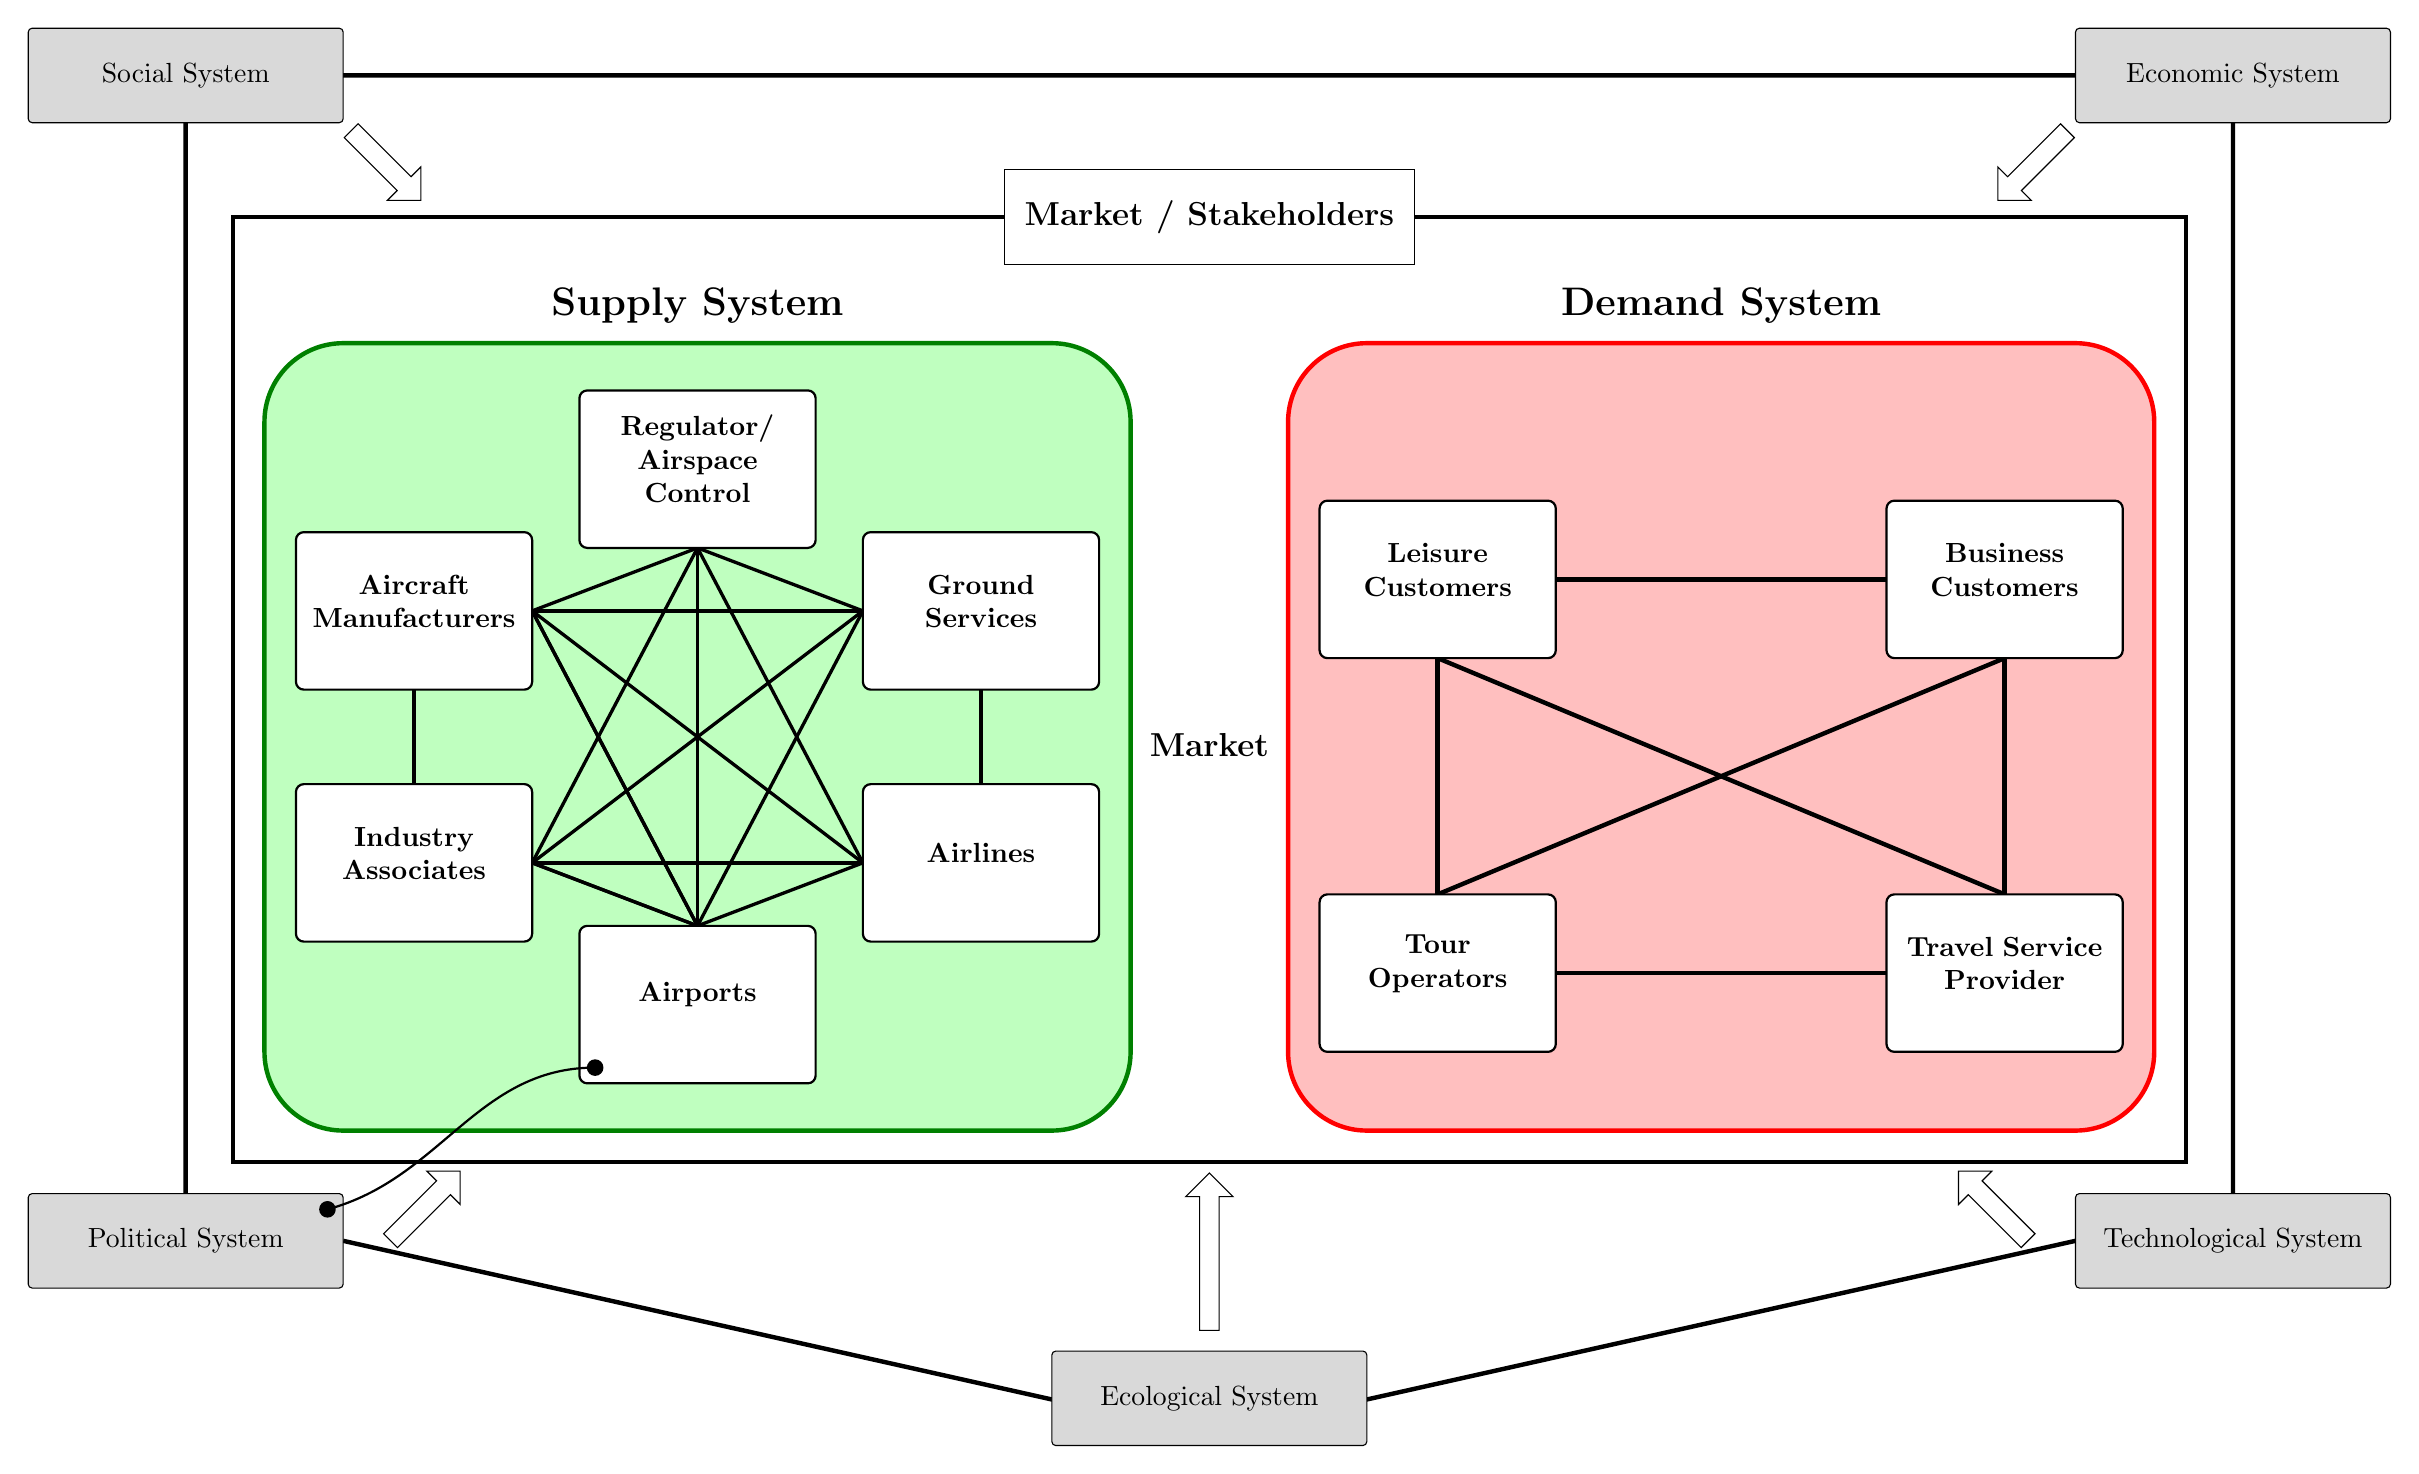
\begin{tikzpicture}
%       \draw[help lines,step=.2,gray!60!white] (0,-2) grid (30,16) ;
        
        % Main Rect
        \draw[ultra thick] (2,.4) -- (2,15.4) -- (28,15.4) -- (28,.6) -- (26,.6) -- (17,-1.415) -- (13,-1.415) -- (4,.6);
        
        
        % Draw inner rects
        \draw[ultra thick] (2.6,1.6) rectangle ++(24.8,12);
        \draw[ultra thick,green!50!black,fill=green!25!white,rounded corners=1cm] (3,2) rectangle ++(11,10);
        \draw[ultra thick,red,fill=red!25!white,rounded corners=1cm] (16,2) rectangle ++(11,10);

        
        % Rects titles
        \draw[draw=black,fill=white] (12.4,13) rectangle ++(5.2,1.2) node [pos=.5]{\textbf{\large Market / Stakeholders}};
        \draw[white] (3,12.1) rectangle ++(11,.75) node[text=black,pos=.5]  {\textbf{\Large Supply System}};
        \draw[white] (16.0,12.1) rectangle ++(11,.75) node[text=black,pos=.5]  {\textbf{\Large Demand System}};
        \draw[white] (14.1,6.4) rectangle ++(1.8,1) node[text=black,pos=.5]  {\textbf{\large Market}};
        
        % Draw inner inner recs (Red)
        \draw[black, ultra thick]  (17.9,4) -- (17.9,9) -- (25.1,9) -- (25.1,4) -- (17.9,4);
        \draw[black, ultra thick]  (17.9,5) -- (25.1,8);
        \draw[black, ultra thick]  (17.9,8) -- (25.1,5);
        \node[fit={(16.4,5) (19.4,3)}, inner sep=0pt,fill=white, draw=black, thick,align=center,rounded corners=.1cm] 
        (rect) {\textbf{Tour\\ Operators}};
        \node[fit={(16.4,8) (19.4,10)}, inner sep=0pt,fill=white, draw=black, thick,align=center,rounded corners=.1cm] (rect) {\textbf{Leisure\\Customers}};
        \node[fit={(23.6,8) (26.6,10)}, inner sep=0pt,fill=white, draw=black, thick,align=center,rounded corners=.1cm] (rect) {\textbf{Business\\Customers}};       
        \node[fit={(23.6,5) (26.6,3)}, inner sep=0pt,fill=white, draw=black, thick,align=center,rounded corners=.1cm] (rect) {\textbf{Travel Service\\Provider}};
        
        
        
        
        % Draw inner inner recs (Green)
    
        
        \draw[black, very thick]  (6.4,8.6) -- (8.5,9.4);
        \draw[black, very thick]  (6.4,8.6) -- (10.6,8.6);
        \draw[black, very thick]  (6.4,8.6) -- (10.6,5.4);
        \draw[black, very thick]  (6.4,8.6) -- (8.5,4.6);
        \draw[black, very thick]  (4.9,7.6) -- (4.9,6.4);
        
        \draw[black, very thick]  (6.4,5.4) -- (8.5,9.4);
        \draw[black, very thick]  (6.4,5.4) -- (10.6,8.6);
        \draw[black, very thick]  (6.4,5.4) -- (10.6,5.4);
        \draw[black, very thick]  (6.4,5.4) -- (8.5,4.6);
        
        \draw[black, very thick]  (8.5,4.6) -- (8.5,9.4);
        \draw[black, very thick]  (8.5,4.6) -- (10.6,8.6);
        \draw[black, very thick]  (8.5,4.6) -- (10.6,5.4);
        \draw[black, very thick]  (8.5,4.6) -- (6.4,8.6);
        \draw[black, very thick]  (8.5,4.6) -- (6.4,5.4);       
        
        \draw[black, very thick]  (10.6,5.4) -- (8.5,9.4);
        \draw[black, very thick]  (10.6,8.6) -- (8.5,9.4);
        \draw[black, very thick]  (12.1,7.6) -- (12.1,6.4);
        
        
        \node[fit={(3.4,4.4) (6.4,6.4)}, inner sep=0pt,fill=white, draw=black, thick,align=center,rounded corners=.1cm] 
        (rect) {\textbf{Industry\\Associates}};
        \node[fit={(3.4,7.6) (6.4,9.6)}, inner sep=0pt,fill=white, draw=black, thick,align=center,rounded corners=.1cm] (rect) {\textbf{Aircraft\\Manufacturers}};
        \node[fit={(10.6,7.6) (13.6,9.6)}, inner sep=0pt,fill=white, draw=black, thick,align=center,rounded corners=.1cm] (rect) {\textbf{Ground\\Services}};       
        \node[fit={(10.6,4.4) (13.6,6.4)}, inner sep=0pt,fill=white, draw=black, thick,align=center,rounded corners=.1cm] (rect) {\textbf{Airlines}};

        \node[fit={(7,2.6) (10,4.6)}, inner sep=0pt,fill=white, draw=black, thick,align=center,rounded corners=.1cm] (rect) {\textbf{Airports}};
        \node[fit={(7,9.4) (10,11.4)}, inner sep=0pt,fill=white, draw=black, thick,align=center,rounded corners=.1cm] (rect) {\textbf{Regulator/\\Airspace\\Control}};

        
        % The four cornered rects {Social syetem, Politcial system, etc.}
        \draw[draw=black,rounded corners=.05cm,fill=gray!30!white] (0,0) rectangle ++(4,1.2) node [pos=.5]{Political System};
        \draw[draw=black,rounded corners=.05cm,fill=gray!30!white] (0,14.8) rectangle ++(4,1.2) node[pos=.5]{Social System};
        \draw[draw=black,rounded corners=.05cm,fill=gray!30!white] (26,14.8) rectangle ++(4,1.2) node[pos=.5]{Economic System};
        \draw[draw=black,rounded corners=.05cm,fill=gray!30!white] (26,0) rectangle ++(4,1.2) node[pos=.5]{Technological System};
%--------------------------------------------------%
        \node [circle, fill=black,inner sep=0pt,minimum size=6pt] (0) at (3.8, 1) {};
        \node [circle, fill=black,inner sep=0pt,minimum size=6pt] (1) at (7.2, 2.8) {};
        \draw [in=-180, out=15, thick] (0.center) to (1.center);
%--------------------------------------------------%
        % Bottom rect of the whole drawing (Ecological System)
        \draw[draw=black,rounded corners=.05cm,fill=gray!30!white] (13,-2) rectangle ++(4,1.2) node [pos=.5]{Ecological System};
        
        % Three outlined arrow in the bottom
        \node at (15,.4) [draw=black,single arrow, minimum width = 14pt, single arrow head extend=5pt,minimum height=20mm,rotate=90] {};
        \node at (5,1) [draw=black,single arrow, minimum width = 14pt, single arrow head extend=5pt,minimum height=12.5mm,rotate=45] {};
        \node at (25,1) [draw=black,single arrow, minimum width = 14pt, single arrow head extend=5pt,minimum height=12.5mm,rotate=135] {};
        \node at (25.5,14.3) [draw=black,single arrow, minimum width = 14pt, single arrow head extend=5pt,minimum height=12.5mm,rotate=225] {};
        \node at (4.5,14.3) [draw=black,single arrow, minimum width = 14pt, single arrow head extend=5pt,minimum height=12.5mm,rotate=315] {};
                
    \end{tikzpicture}    
\end{document}